\documentclass{scrreprt}

\usepackage{aligned-overset}
\usepackage{amsmath}
\usepackage{amssymb}
\usepackage{bm}
\usepackage[shortlabels]{enumitem}
\usepackage{hyperref}
\usepackage[utf8]{inputenc}
\usepackage{multicol}
\usepackage{mathtools}
\usepackage{physics}
\usepackage{pdflscape}
\usepackage{tabularx}
\usepackage{titling}
\usepackage{fancyhdr}
\usepackage{xfrac}
\usepackage[dvipsnames]{xcolor}
\usepackage{pgfplots}

\pgfplotsset{compat = newest}
\usetikzlibrary{intersections}
\usetikzlibrary{patterns}
\usepgfplotslibrary{fillbetween}

\author{Karsten Lehmann (Übungsgruppe 1)\\Mat. Nr 4935758}
\date{WiSe 2021/2022}
\title{Hausaufgaben Blatt 13\\Analysis - Grundlegende Konzepte}

\setlength{\headheight}{26pt}
\pagestyle{fancy}
\fancyhf{}
\lhead{\thetitle}
\rhead{\theauthor}
\lfoot{\thedate}
\rfoot{Seite \thepage}

\begin{document}
\paragraph{69. Im Folgenden sollen Sie ein Additionstheorem für die Tangensfunktion beweisen}
\begin{enumerate}[(a)]
\item Seien $x, y \in \mathbb{R} \setminus \qty{k\pi + \frac{\pi}{2}
    \,\middle|\, k \in \mathbb{Z}}$.
  Bestimmen Sie $y$ in Abhängigkeit von $x$, sodass die Gleichung
  \[
    \tan\qty\big(x)\tan\qty\big(y) = 1
  \]
  gilt.
  Welche Bedingung erfüllt $x + y$.

  \subparagraph{Lsg.} Es ist $\tan x = \frac{\sin x}{\cos x}$ für
  $x \in \mathbb{R} \setminus \qty{\frac{\pi}{2} + k\pi
    \,\middle|\, k \in \mathbb{Z}}$ und
  $\cos\qty\big(x + y) = \cos x \cos y - \sin x \sin y$.
  \begin{flalign*}
    \tan\qty\big(x)\tan\qty\big(y) &= 1 &&\iff \\
    \frac{\sin x}{\cos x} \cdot \frac{\sin y}{\cos y} &= 1
    &&{\Big |} \cdot \frac{\cos y}{\sin y} \\
    \frac{\sin x}{\cos x} &= \frac{\cos y}{\sin y} \\
    \sin x \sin y &= \cos x \cos y \\
    0 &= \cos x \cos y - \sin x \sin y \\
    0 &= \cos\qty\big(x + y) &\overset{\text{Satz 13.20}}&\iff \\
    x + y &= \frac{pi}{2} + k\pi, k \in \mathbb{Z}
  \end{flalign*}

  $\Rightarrow$ \underline{$y = \frac{pi}{2} + k\pi - x$, $k \in \mathbb{Z}$}.

\item Es seien $x, y \in \mathbb{R} \setminus \qty{k\pi + \frac{\pi}{2}
    \,\middle|\, k \in Z}$.
  Beweisen Sie, dass
  \[
    \tan\qty\big(x + y) = \frac{\tan\qty\big(x) + \tan\qty\big(y)}
    {1 - \tan\qty\big(x)\tan\qty\big(y)}
  \]

  \subparagraph{Lsg.}
  \begin{flalign*}
    \frac{\sin\qty\big(x + y)}{\cos\qty\big(x + y)}
    &= \frac{\frac{
        \sin x}{\cos x} + \frac{\sin y}{\cos y}
    }{
      1 - \frac{\sin x}{\cos x}\frac{\sin y}{\cos y}
    } && {\Big |}\, \cdot \cos x \cos y\\
    &= \frac{\sin x \cos y + \sin y \cos x}{\cos x \cos y - \sin x \sin y} \\
    \overset{\text{Satz 13.15 (4)}}&=
    \frac{\sin\qty\big(x + y)}{\cos\qty\big(x + y)}
  \end{flalign*}
\end{enumerate}

\newpage
\paragraph{70. In dieser Aufgabe sollen Sie die Anwendung der Polarkoordinaten
  komplexer Zahlen üben.}
\begin{enumerate}[(a)]
\item Geben Sie mit Hilfe der Exponentialdarstellung einer Zahl
  $z \in \mathbb{C}$ eine geometrische Interpretation der Multiplikation
  in $\mathbb{C}$ in der komplexen Zahlebene.

  \subparagraph{Lsg.} Seien $z_1, z_2 \in \mathbb{C}$ und
  $\xi_1, \xi_2 \in \big[0, 2\pi\big)$ so gewählt, dass
  $z_1 = \abs{z_1} \cdot e^{\xi_1 \cdot i}$ und
  $z_2 = \abs{z_2} \cdot e^{\xi_2 \cdot i}$.

  Nun ist $z_1 \cdot z_2 = \abs{z_1} e^{i \xi_1} \cdot \abs{z_2} e^{i \xi_2}
  = \abs{z_1 z_2} e^{i\qty\big(\xi_1 + \xi_2)}$.

  \begin{tikzpicture}[scale=1.5]
    \begin{axis}[
      axis x line=center,
      axis y line=center,
      grid=both,
      xlabel={Re},
      xmin=-2.1,
      xmax=2.1,
      xticklabels={,,},
      ylabel={Im},
      ymin=-2.1,
      ymax=2.1,
      yticklabels={,,},
    ]
      \node[circle, fill, label=right:{$z_1$}, inner sep=2pt] at (0.5,1) {};
      \node at (0.2, 0.1) {\tiny $\xi_1$};
      \node[black!70!green, circle, fill, label=above:{$z_2$}, inner sep=2pt] at (-0.4,0.4) {};
      \node[black!70!green] at (-0.07, 0.2) {\tiny $\xi_2$};
      \node[black!50!red, circle, fill, label=below:{$z_1 \cdot z_2$}, inner sep=2pt] at (-1.74,-0.57) {};
      \node[black!50!red] at (-1.3, 0.5) {\tiny $\xi_1 + \xi_2$};

      \draw (0,0) -- (0.5,1) node[right, pos=.5] {\tiny $\abs{z_1}$};
      \draw (0.3,0) arc (0:64:0.3);

      \draw[black!70!green] (0,0) -- (-0.4,0.4) node[below left = -3pt, black!70!green, pos=.5] {\tiny $\abs{z_2}$};
      \draw[black!70!green] (0.35,0) arc (0:135:0.35);

      \draw[black!50!red] (0,0) -- (-1.74,-0.57) node[below=4pt, black!50!red, pos=.5] {\small $\abs{z_1 + z_2}$};
      \draw[black!50!red] (1,0) arc (0:198:1);
    \end{axis}
  \end{tikzpicture}
\end{enumerate}
\end{document}
